\section{Dataset 15\%}

In this section we present the datasets we have used: one for the detection task and one for the classifier models. 

\subsection{Dataset for the detector}
For training the detector model using the YOLO algorithm, we built our own dataset. Firstly, we extracted a hundred JPG images from the DFG Traffic Sign Dataset\footnote{\url{http://www.vicos.si/Downloads/DFGTSD}} which consists of about 7000 images with 1920x1080 resolution captured in Slovenian roads. The RGB images were acquired with a camera mounted on a vehicle that was driven through six different Slovenian municipalities. The image data was acquired in rural as well as urban areas. Each image contains at least one traffic sign. After that, using a utility tool we manually selected for each image the coordinates of the position where the traffic signs are located. In such way, for each image in the training set there is a .txt file that indicates in each row the position of the traffic signs. To locate target objects we used the YOLO bounding box format (0, x-top left, y-top left, width, height) where 0 represents the class of the object (the model has only to detect the traffic signs location), x and y represent the coordinates of the top left corner, width and height represent the object dimensions. For testing this model we've taken other images from the same dataset. The same was done to build the validation set.


\subsection{Dataset for the classifier}
The Belgium Traffic Sign Dataset\footnote{\url{https://btsd.ethz.ch/shareddata}} refers to a set of 62 classes of traffic signs: training data files are divided into 62 folders that contain the images in PPM format. The same for validation data. We decided to cut some classes and to add some new ones in order to build an accurate classifier which focuses on most meaningful traffic signs. For some classes the number of images was too low to obtain a good result, so we merged this dataset with some images taken from the German Traffic Sign Recognition Benchmark\footnote{\url{http://benchmark.ini.rub.de}}, a dataset made for a multi-class image classification benchmark in the domain of advanced driver assistance systems and autonomous driving. The dataset we have used to train and to validate the classifier model is made of 56 traffic sign classes with 6229 images for training and 2493 for the validation. Every image is a cropped portion taken from a road picture which represents one traffic sign. Typically the images are characterized by small square sizes. The aim of the classifier is to pick the right class for each input image, but in Europe there could be small appearance differences between the same traffic sign classes from a country to another. 
\begin{figure}{}
	\centering
	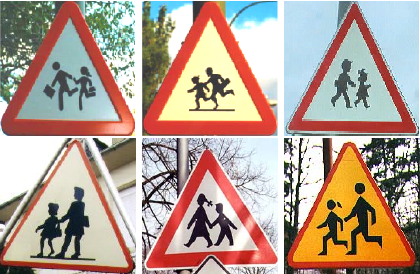
\includegraphics[width=0.6\linewidth]{Res/Immagini/differences.png}
	\caption{Differences between signs of the same class}\label{}
\end{figure}
To fix this issue, we manually added some images to training and validation data for classes which suffer this problem. Also, we adopted the augmentation technique to build a more generalized dataset and to prevent the overfitting problem. We added small variations to the input images introducing rotation by 10\%, width and height resizing, shearing and zooming randomly up to a tenth. It is important to not exaggerate with the changes because it could cause problem with the classification, due to the fact that some signs have specific orientation.

\subsection{Custom made test dataset}
The application is supposed to work in real-time situations and for this reason we recorded some videos using a front car camera. For video recording we have used an iPhone XR setting the quality on 1080p and 30 fps. We've taken short videos, from 30 seconds to a minute, for testing how good the combination of the detector and the classifier works.